\section*{Experiment 3}

Differential ampl


\subsection*{Large Signal Analysis}

% Is the response symmetrical? You will probably notice that the output
% of the amplifier follows a linear trajectory in time over most of its response to the large input
% step. This behavior is called slewing, and the constant rate of change of the output voltage
% with respect to time is called the slew rate of the amplifier. Extract a slew rate for both for
% the up-going and for the down-going output transitions. How do these compare with those
% which you compute from the load capacitance and the limiting values of the output current?
% In your report, include a single plot showing both scope traces along with the extracted slew
% rates.

\begin{figure}[H]
\centering
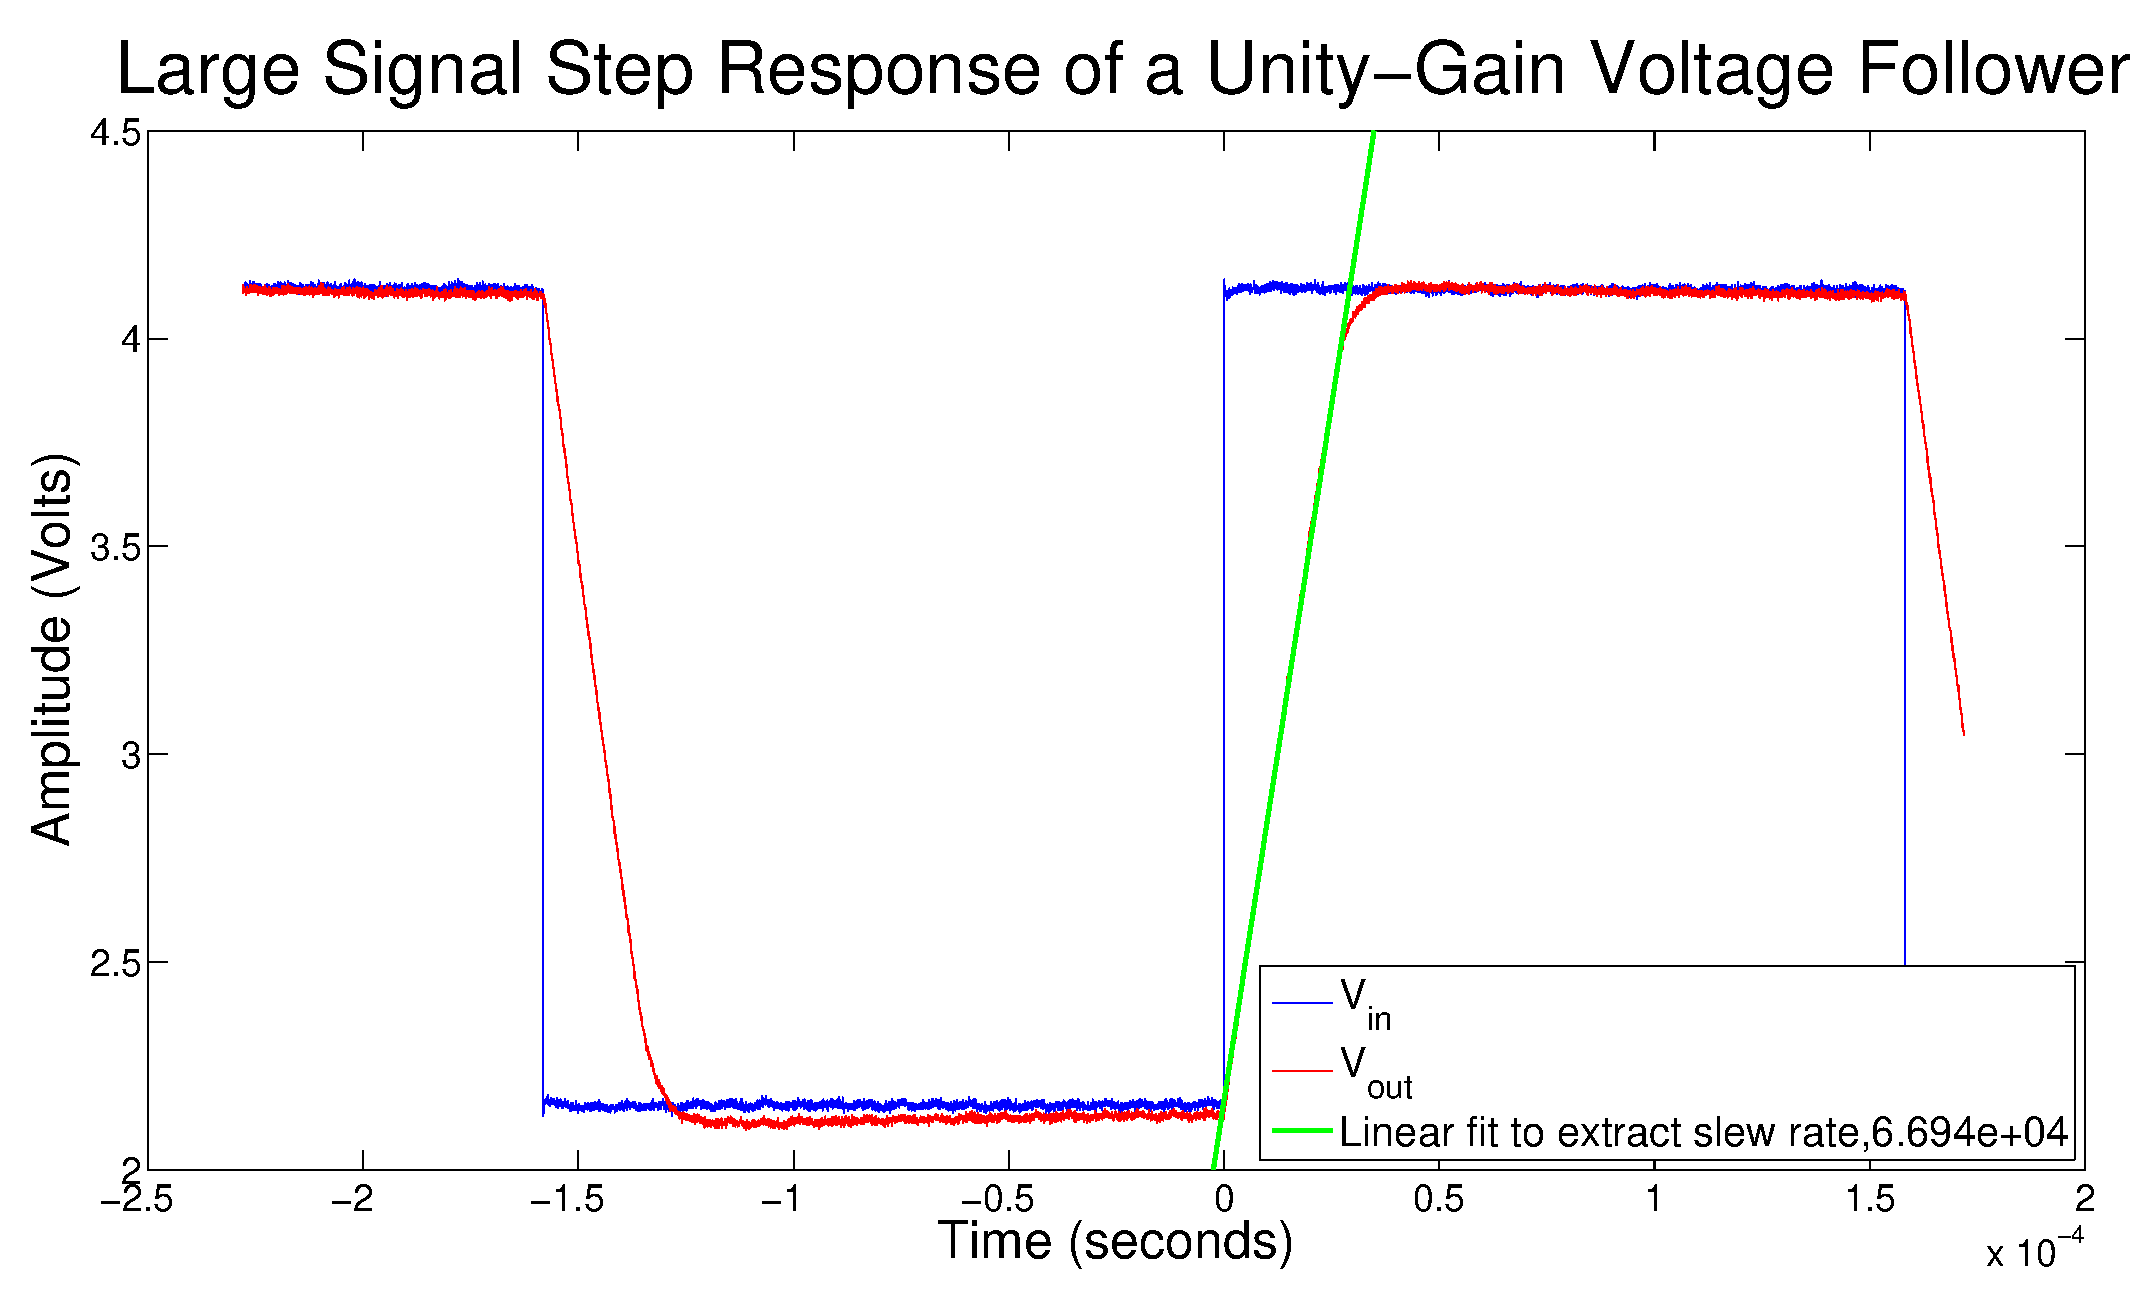
\includegraphics[width=\linewidth]{../Figures/Exp3P1.eps}
\caption{}
\label{fig:exp3p1}
\end{figure}

\subsection*{Small Signal Analysis}

% Is the response symmetrical? Does the amplifier exhibit approximately
% linear behavior? Extract a time constant both for the up-going and for the down-going
% output transitions. How do these compare with that which you compute from the measured
% values of the load capacitance and the differential-mode transconductance gain that you
% found in Experiment 2? In your report, include a single plot showing both scope traces
% along with the extracted time constants.


\begin{figure}[H]
\centering
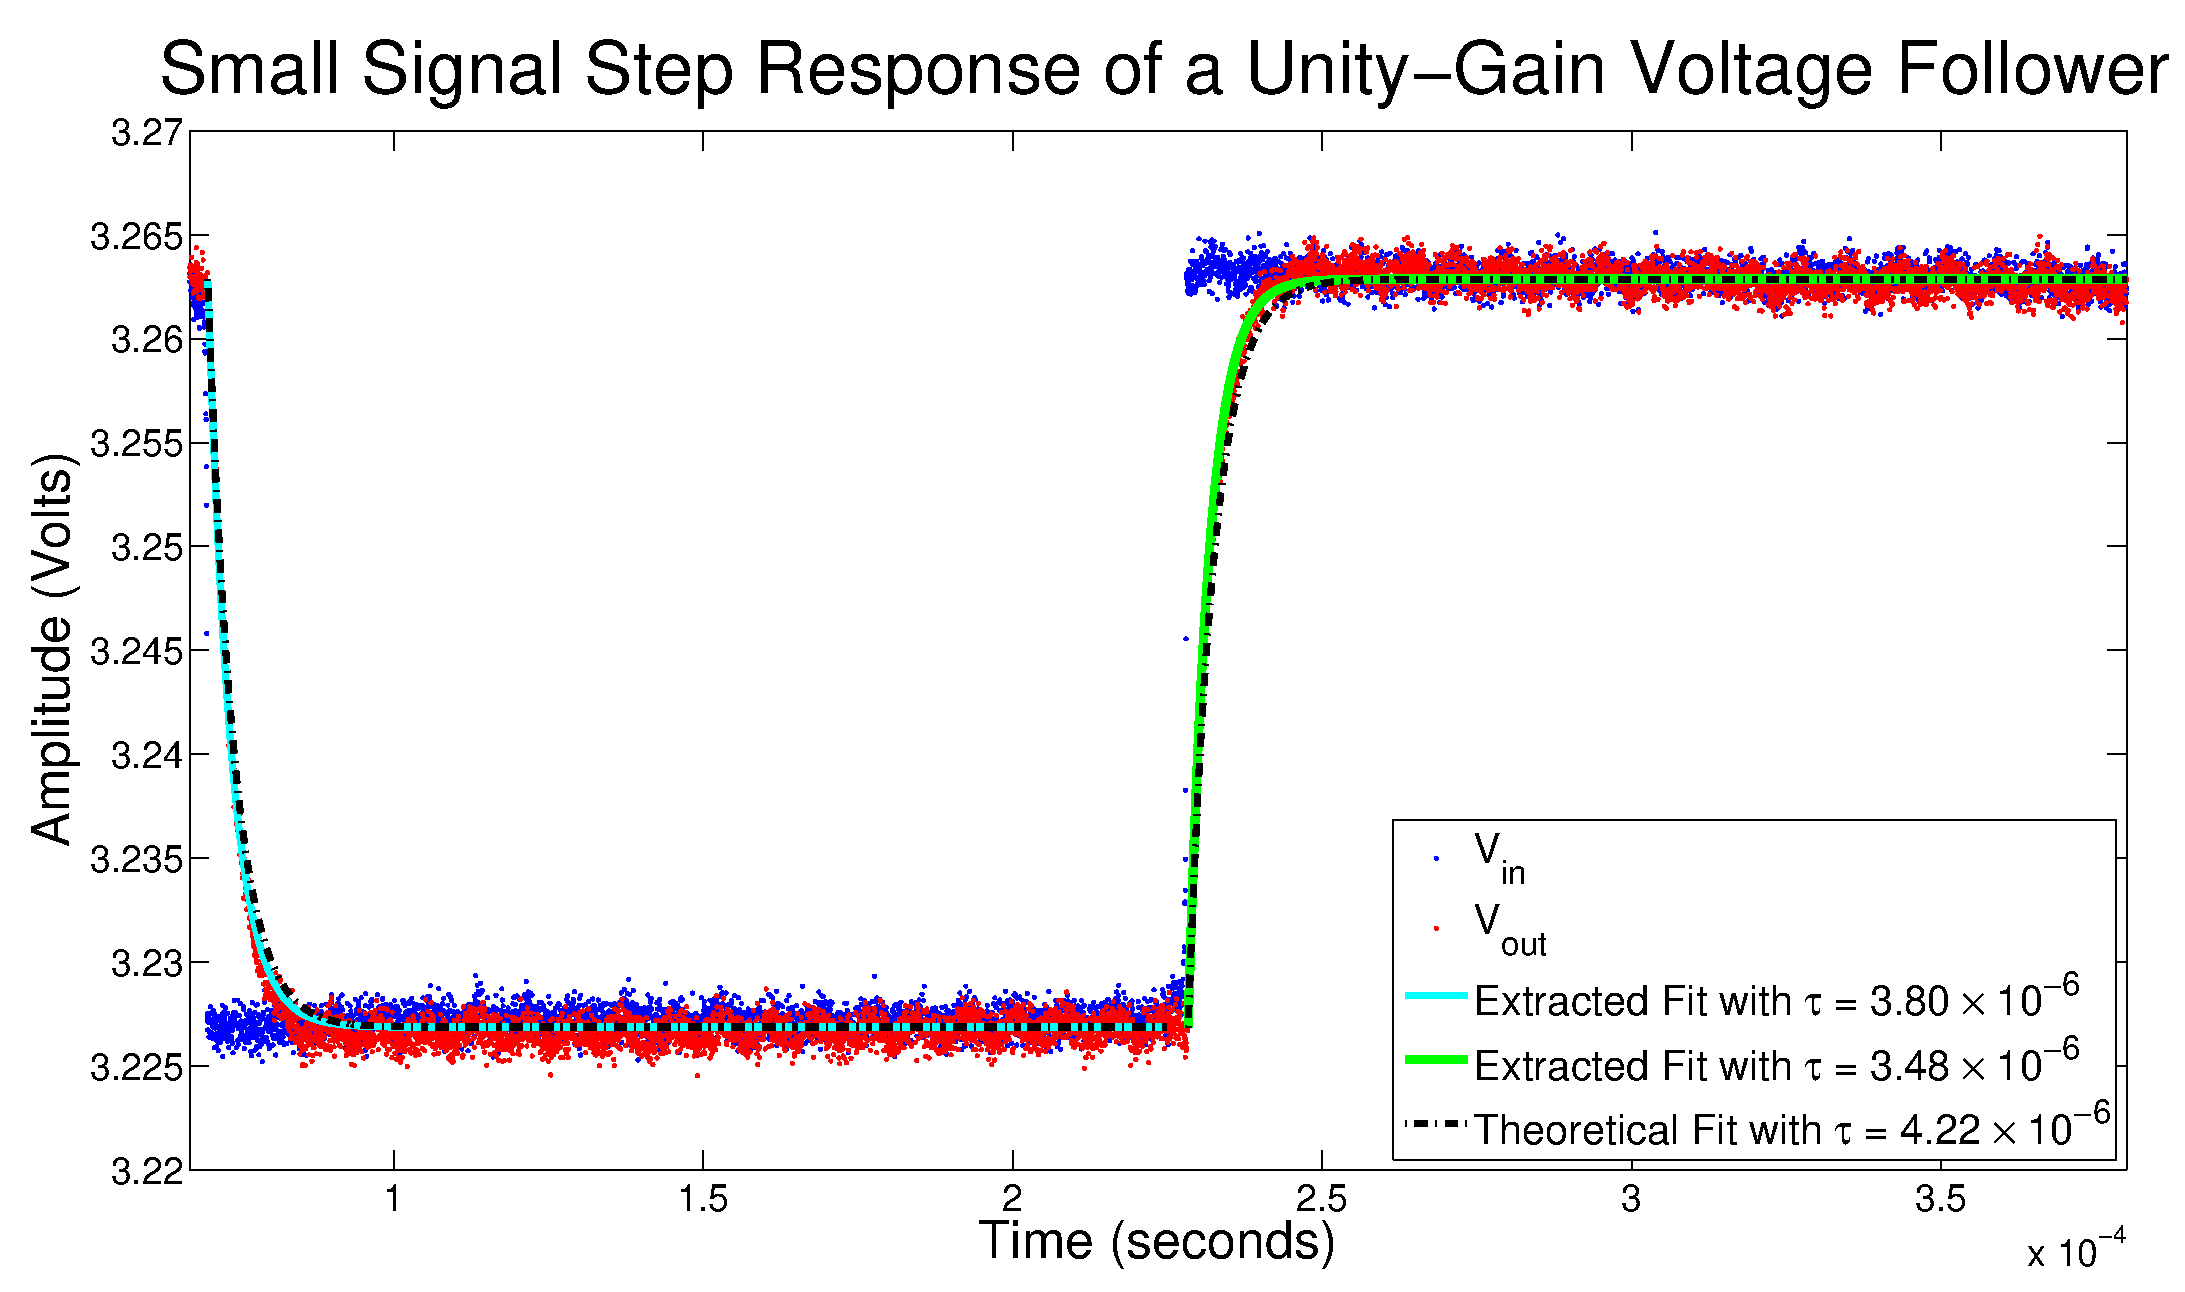
\includegraphics[width=\linewidth]{../Figures/Exp3P2.eps}
\caption{}
\label{fig:exp3p2}
\end{figure}